\chapter{Implementasjon}

\textbf{En kort sammenstilling av de elementer som er implementert fra oppgaveteksten og utøver.}

\section{Fragment}
Det benyttes fragmenter fremst in listen for alle kontakter som er presentert i figur \ref{fig:liste_fragment}, side \pageref{fig:liste_fragment}. Listefragmentet bruker en egen layout fil i to versjon for liggende og stående orientering.
Andre fragmenter som også benyttes er dialog fragment i form av en bekreftelse ved lagring eller endring av en kontakt. 
Det siste fragmentet som brukes er preferance fragment der det brukes standard oppsett av en preferance liste som finnes i systemet (figur \ref{fig:preferance_fragment}, side \pageref{fig:preferance_fragment}). 
Alle innstillinger som blir endret via preference fragmet blir lagret og lest fra \texttt{SharedPreferences}.

\section{Inputvalidering}
Det blir validert input for navn og telefonnummer. Navn blir validert slik at feltet kan ikke være tomt og får kun innhole bokstaver. 
Feltet for telefonnummer blir validert med to regex strenger, en som tester på at det er kun tall som brukes og det andre om at lengden på tallrekken får være mellom 8 og 12 tall. Se figur \ref{fig:validering}, side \ref{fig:validering}. Validering blir kjørt først når brukeren klikker videre i action baren.  

\section{Navigering}
All navigering i applikasjonen gjøres fra action bar. Det finnes ingen andre knapper eller liknende i aktivitetene uten alt blir styrt direkte fra action bar hvilket gir samme enhetlig følelse tvers over hele applikasjonen. 

\section{Database}
Det benyttes en \texttt{sqlite} database med kolonner som motsvarer alle de felt som finnes i Person objektet. Disse er id, navn, melding til personen, dato for bursdag, tid for individuell utsendelse av melding (benyttes ikke), \texttt{erAktiv} (dersom man ønsker at melding service skal være aktiv eller ikke til den personen). Person objekter opprettes fra databasen gjennom vanlige sql spørringer. Det samme gjelder også for lagring. 


\section{Services og BroadcastReceiver}
I applikasjonen brukes det totalt to servicer og en \texttt{BroadcastReceiver} som kaller opp første hovedservicen etter oppstart av telefonen. Dette medfører at applikasjonen trenger ikke startes uten service kommer til å starte automatisk ved systemstart. Hovedservicen kjører hele tiden og ved valgt klokkeslett starter den en sekundær service som ser etter hvilke kontakter i databasen som har bursdag under den aktuelle dagen. Dersom slike personer finnes blir det sendt meldinger med den forhåndsdefinerte teksten. 
Når hovedservicen kjører vises det en notifikasjon i telefonens info felt (se figur \ref{fig:notification}, side \pageref{fig:notification}).

\section{Content provider}
\texttt{ContentPrivider} er implementert slik at data som tilhører \texttt{Birthday-o-Matic} er tilgjengelig til andre applikasjoner i systemet. Content provideren er bygget opp gjennom at man benytter seg av direkte spørringer som returnerer \textit{collections} med person objekter i \texttt{DBHandler} klassen. Sammen med prosjektet er det også levert inn en testapplikasjon som gjør det mulig å teste denne funksjonen (se figur \ref{fig:content_provider}).

\begin{figure}[ht]
    \centering
    \begin{subfigure}[b]{0.35\textwidth}
        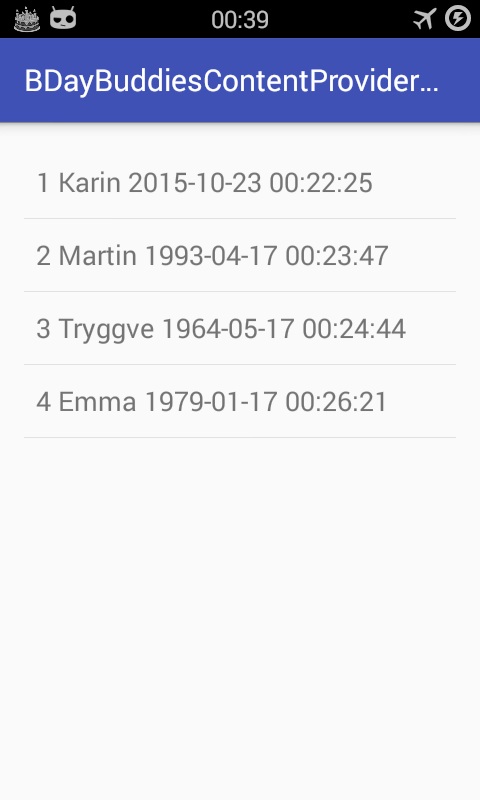
\includegraphics[width=\textwidth]{./img/11.png}
        \caption{Testapp for ContentProvider}
        \label{fig:test_content_provider}
    \end{subfigure}
    \begin{subfigure}[b]{0.35\textwidth}
        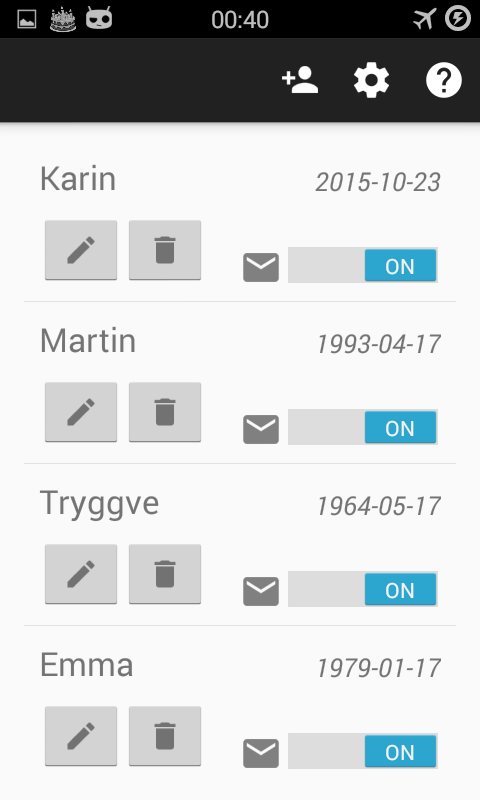
\includegraphics[width=\textwidth]{./img/12.png}
        \caption{Gjenspeiler data i hovedappen}
        \label{fig:test_hovedapp}
    \end{subfigure}
    \caption{Demo av ContentProvider}
    \label{fig:content_provider}
\end{figure}




\chapter{Aktiviteter}
\textbf{Kapitelet viser en oversikt over alle aktiviteter i applikasjoner. }

Ved oppbyggingen av de grafiske komponentene i applikasjonen har jeg valgt å fokusere på å tilnærme seg så godt som mulig en \textit{native} applikasjon for API 19 gjennom å direkte modifisere standard komponenter uten noen overdreven fargetema eller \textit{custom} fonter. 
Tanken er at brukeren skal kjenne seg så mye som mulig fra en standard kontaktliste applikasjon. 
Jeg utgår fra at slik bursdagsapp blir ikke brukt ofte, kun når kontakter skal legges til eller endres. Appen skal gjøre jobben sin i bakgrunnen derfor er det lagt vekt på at det skal være enkelt å kjenne seg igjen i applikasjonen også hvis man ikke har brukt den på lengre tid. 

Det er i stort sett kun brukt tre farger gjennom hela applikasjonen som er svart, grått og hvitt. Eventuelle input felt er markert med standard turkis farve. Samme gjelder for komponenter som \texttt{Switcher} og \texttt{DatePicker}. Innføring av meldingstext skjer i en \texttt{EditText} som har en egen stil for rammen rundt den komponenten for å fremheve den i form av en editering felt for tekst (standard komponenten er kun en rett horisontal linje).

I dette kapitel presenteres derfor bilder av de viktigste aktivitetene og UIX komponenter som er opprettet for applikasjonen. 

\begin{figure}[ht]
    \centering
    \begin{subfigure}[b]{0.35\textwidth}
        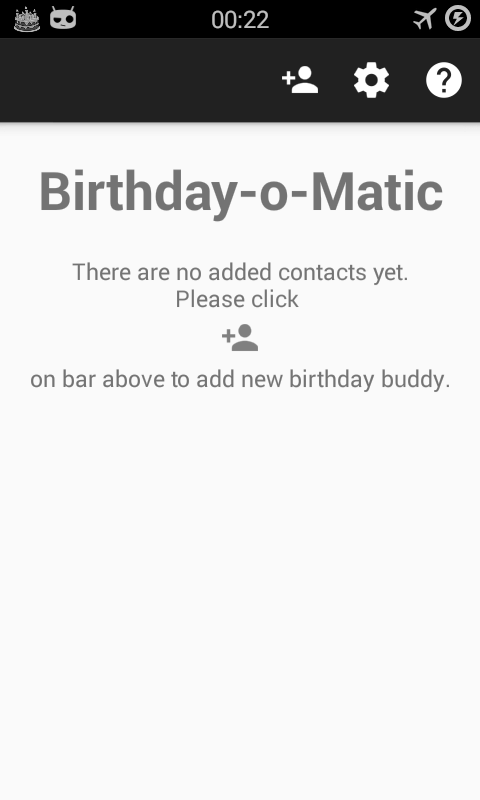
\includegraphics[width=\textwidth]{./img/1.png}
        \caption{Ingen kontakter registrert}
        \label{fig:ingen_kontakter}
    \end{subfigure}
    \begin{subfigure}[b]{0.35\textwidth}
        
\includegraphics[width=\textwidth]{./img/2.png}
        \caption{Ny kontakt}
        \label{fig:ny_kontakt}
    \end{subfigure}
    \begin{subfigure}[b]{0.35\textwidth}
        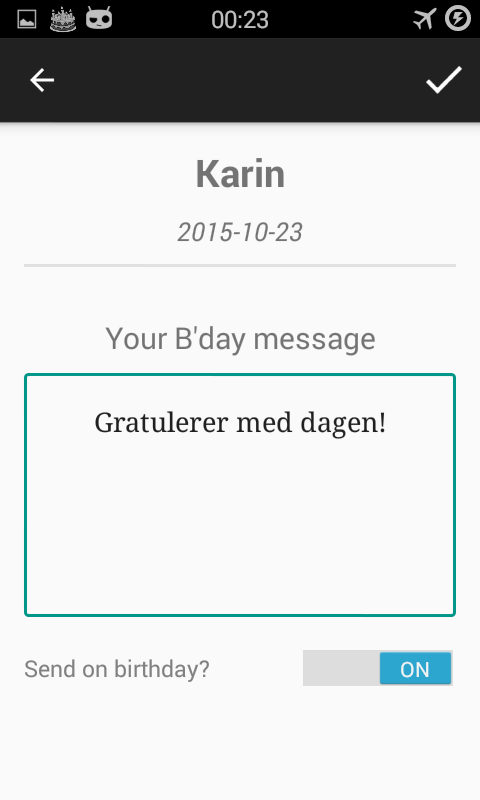
\includegraphics[width=\textwidth]{./img/3.png}
        \caption{Melding}
        \label{fig:melding}
    \end{subfigure}
    \begin{subfigure}[b]{0.35\textwidth}
        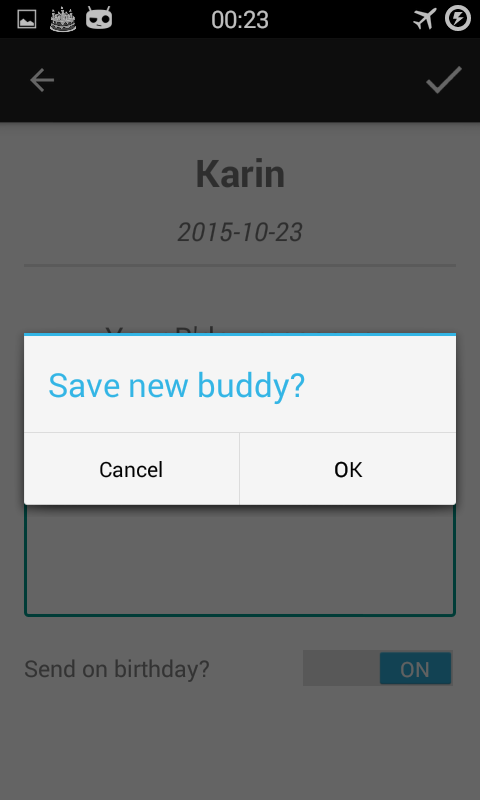
\includegraphics[width=\textwidth]{./img/4.png}
        \caption{Dialog fragment}
        \label{fig:dialog_fragment}
    \end{subfigure}
    \caption{Fremgang for å legge til en ny kontakt.}
    \label{fig:ny_kontakt_workflow}
\end{figure}


\begin{figure}[ht]
    \centering
    \begin{subfigure}[b]{0.35\textwidth}
        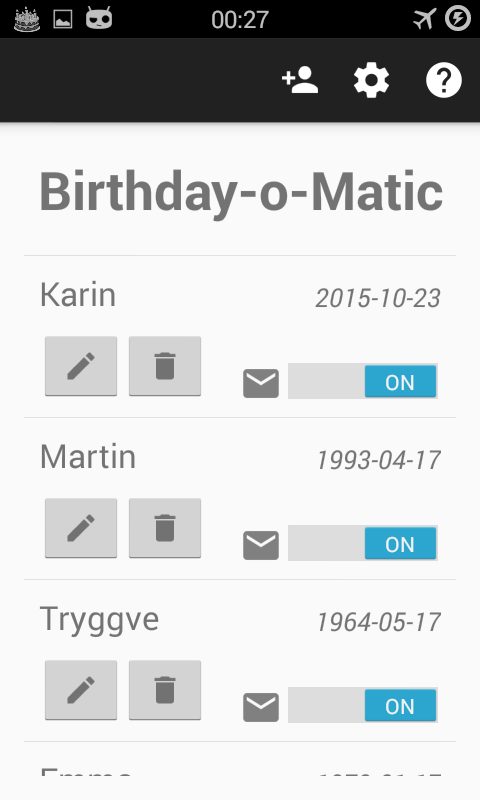
\includegraphics[width=\textwidth]{./img/5.png}
        \caption{Liste fragment (portrait)}
        \label{fig:liste_fragment_p}
    \end{subfigure}
    \begin{subfigure}[b]{0.6\textwidth}
        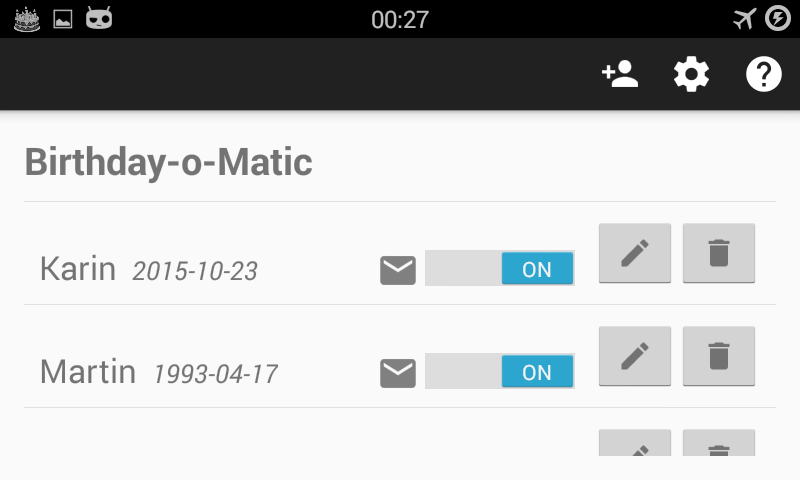
\includegraphics[width=\textwidth]{./img/6.png}
        \caption{Liste fragment (landscape)}
        \label{fig:liste_fragment_l}
    \end{subfigure}
    \caption{Varierende orientering av liste fragment}
    \label{fig:liste_fragment}
\end{figure}


\begin{figure}[ht]
    \centering
    \begin{subfigure}[b]{0.35\textwidth}
        
\includegraphics[width=\textwidth]{./img/2.png}
        \caption{Ny kontakt (portrait)}
        \label{fig:ny_kontakt_p}
    \end{subfigure}
    \begin{subfigure}[b]{0.6\textwidth}
        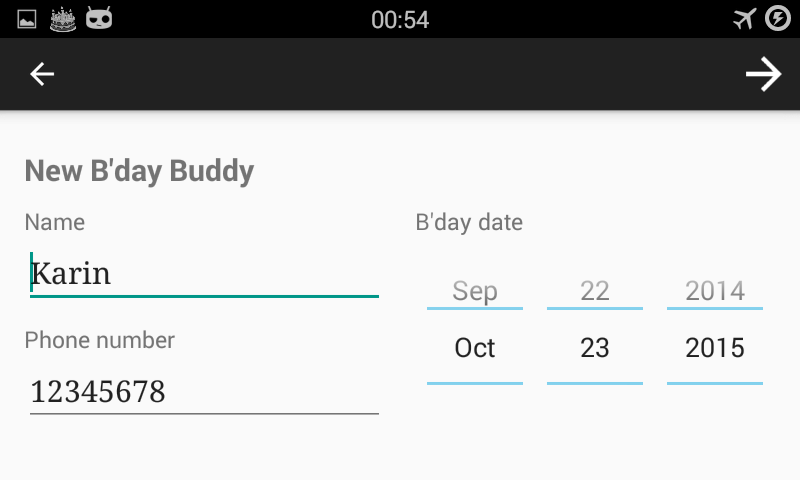
\includegraphics[width=\textwidth]{./img/13.png}
        \caption{Ny kontakt (landscape)}
        \label{fig:ny_kontakt_l}
    \end{subfigure}
    \caption{Orientering av ny kontakt aktivitet}
    \label{fig:ny_kontakt_aktivitet}
\end{figure}

\begin{figure}[ht]
    \centering
    \begin{subfigure}[b]{0.35\textwidth}
        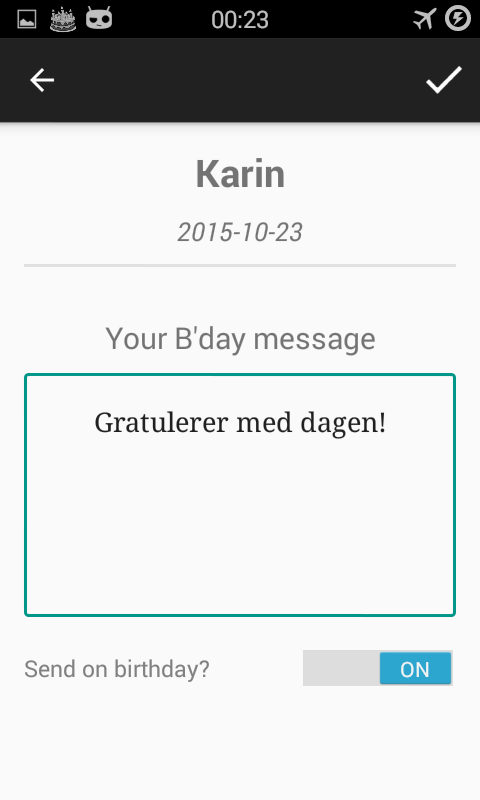
\includegraphics[width=\textwidth]{./img/3.png}
        \caption{Melding (portrait)}
        \label{fig:melding_p}
    \end{subfigure}
    \begin{subfigure}[b]{0.6\textwidth}
        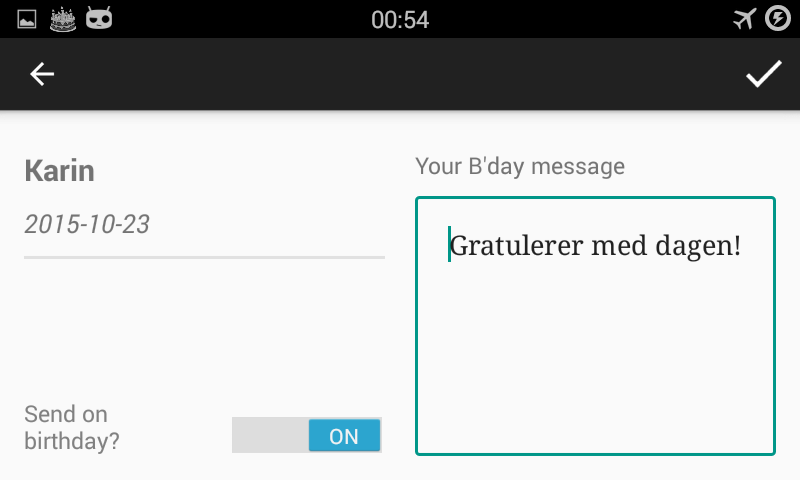
\includegraphics[width=\textwidth]{./img/14.png}
        \caption{Melding (landscape)}
        \label{fig:melding_l}
    \end{subfigure}
    \caption{Orientering av melding aktivitet}
    \label{fig:melding_aktivitet}
\end{figure}

\begin{figure}[ht]
    \centering
    \begin{subfigure}[b]{0.35\textwidth}
        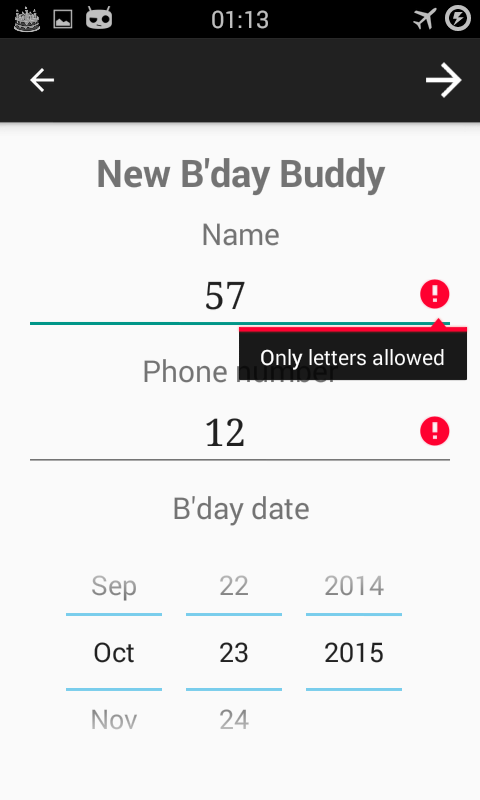
\includegraphics[width=\textwidth]{./img/15.png}
        \caption{Validering av navn}
        \label{fig:validering_tekst}
    \end{subfigure}
    \begin{subfigure}[b]{0.35\textwidth}
        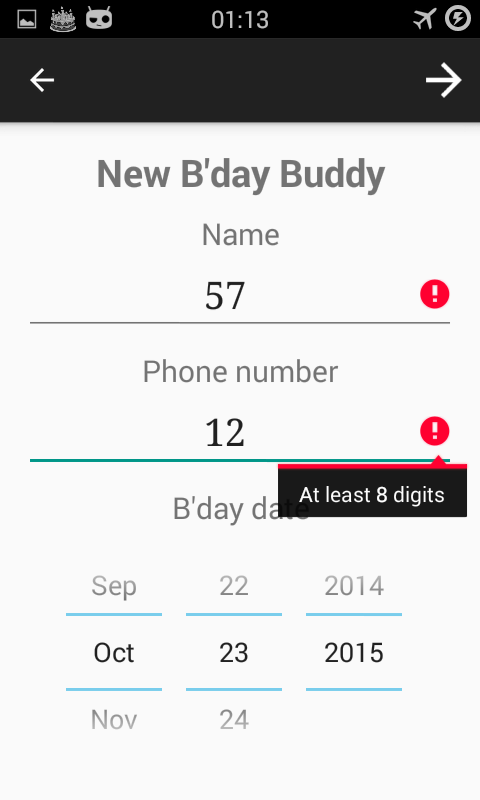
\includegraphics[width=\textwidth]{./img/16.png}
        \caption{Validering av telefonnummer}
        \label{fig:validering_tall}
    \end{subfigure}
    \caption{Inputvalidering}
    \label{fig:validering}
\end{figure}

\begin{figure}[ht]
    \centering
    \begin{subfigure}[b]{0.35\textwidth}
        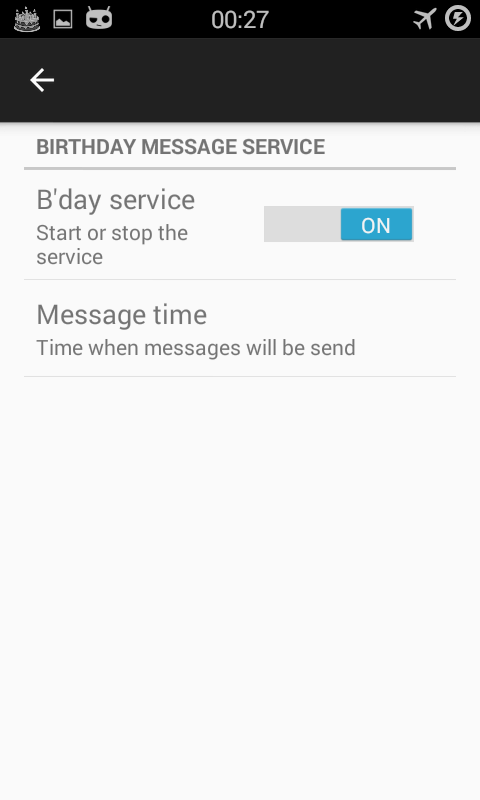
\includegraphics[width=\textwidth]{./img/7.png}
        \caption{Preference fragment}
        \label{fig:preferance_fragment}
    \end{subfigure}
    \begin{subfigure}[b]{0.35\textwidth}
        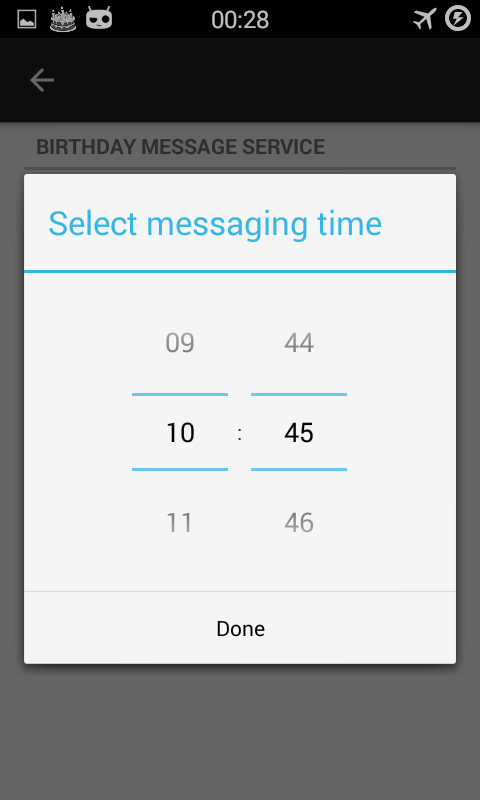
\includegraphics[width=\textwidth]{./img/8.png}
        \caption{Tid for seding}
        \label{fig:melding_tid}
    \end{subfigure}
    \begin{subfigure}[b]{0.35\textwidth}
        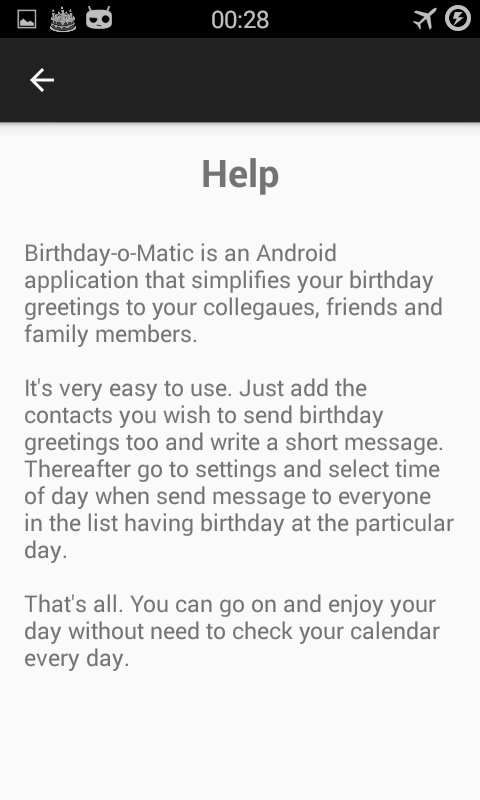
\includegraphics[width=\textwidth]{./img/9.png}
        \caption{Hjelp aktivitet}
        \label{fig:hjelp_aktivitet}
    \end{subfigure}
    \begin{subfigure}[b]{0.35\textwidth}
        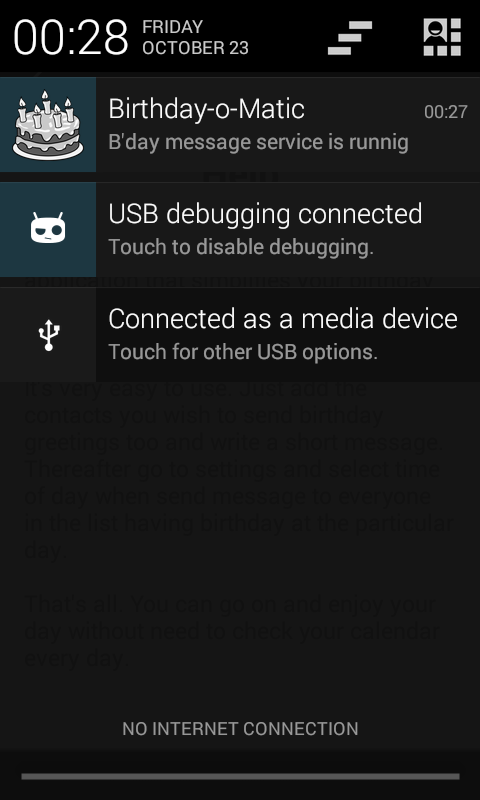
\includegraphics[width=\textwidth]{./img/10.png}
        \caption{Service notification}
        \label{fig:notification}
    \end{subfigure}
    \caption{Øvrige aktiviteter og fragmenter.}
    \label{fig:ovrige_aktiviteter}
\end{figure}


\begin{figure}[ht]
    \centering
    \begin{subfigure}[b]{0.35\textwidth}
        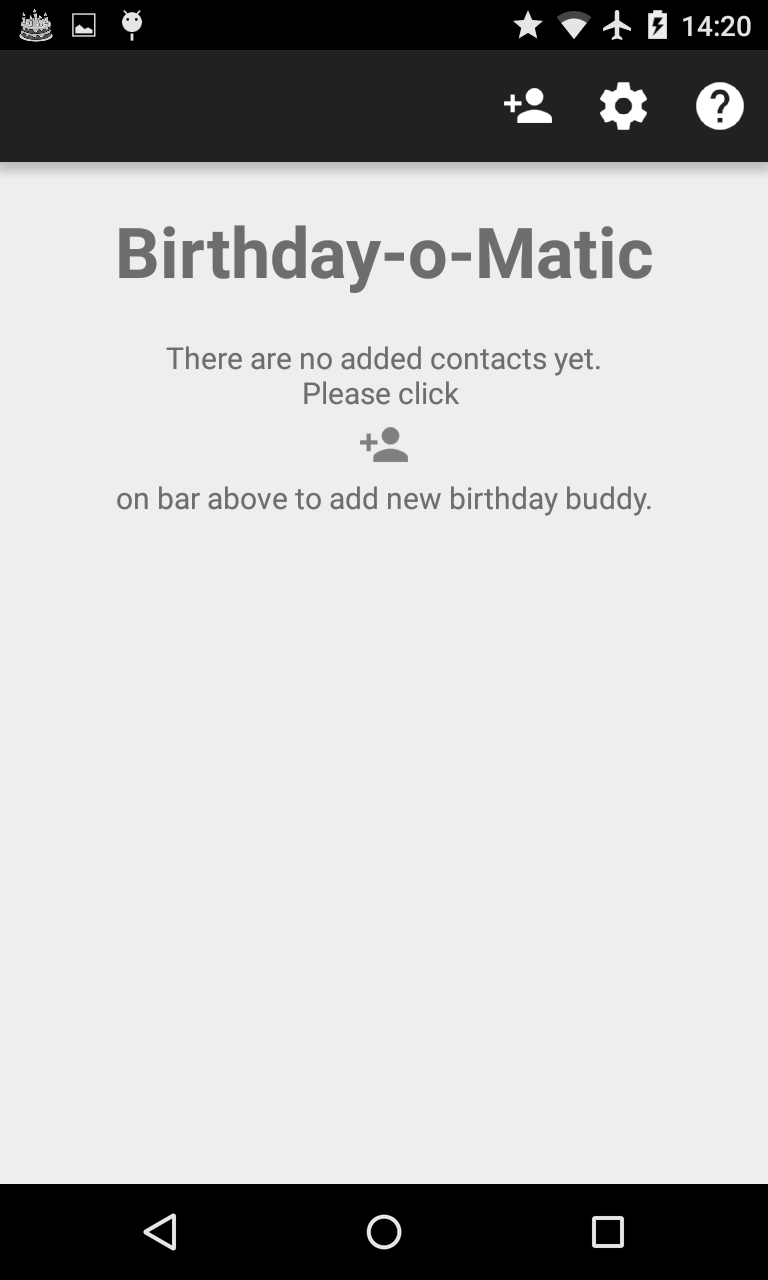
\includegraphics[width=\textwidth]{./img/nexus4/4.png}
        %\caption{Preference fragment}
        \label{fig:res_tom}
    \end{subfigure}
    \begin{subfigure}[b]{0.35\textwidth}
        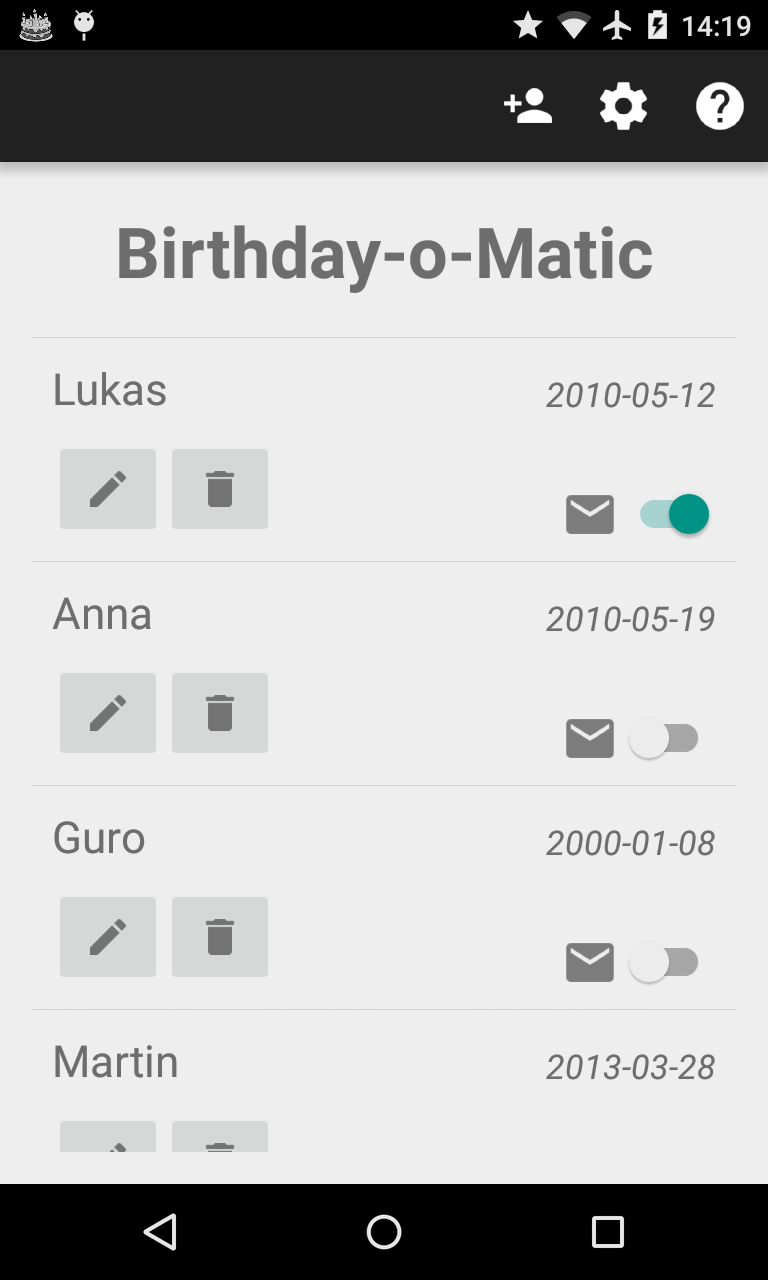
\includegraphics[width=\textwidth]{./img/nexus4/1.png}
        %\caption{Tid for seding}
        \label{fig:res_liste}
    \end{subfigure}
    \begin{subfigure}[b]{0.35\textwidth}
        
\includegraphics[width=\textwidth]{./img/nexus4/2.png}
        %\caption{Hjelp aktivitet}
        \label{fig:res_pers}
    \end{subfigure}
    \begin{subfigure}[b]{0.35\textwidth}
        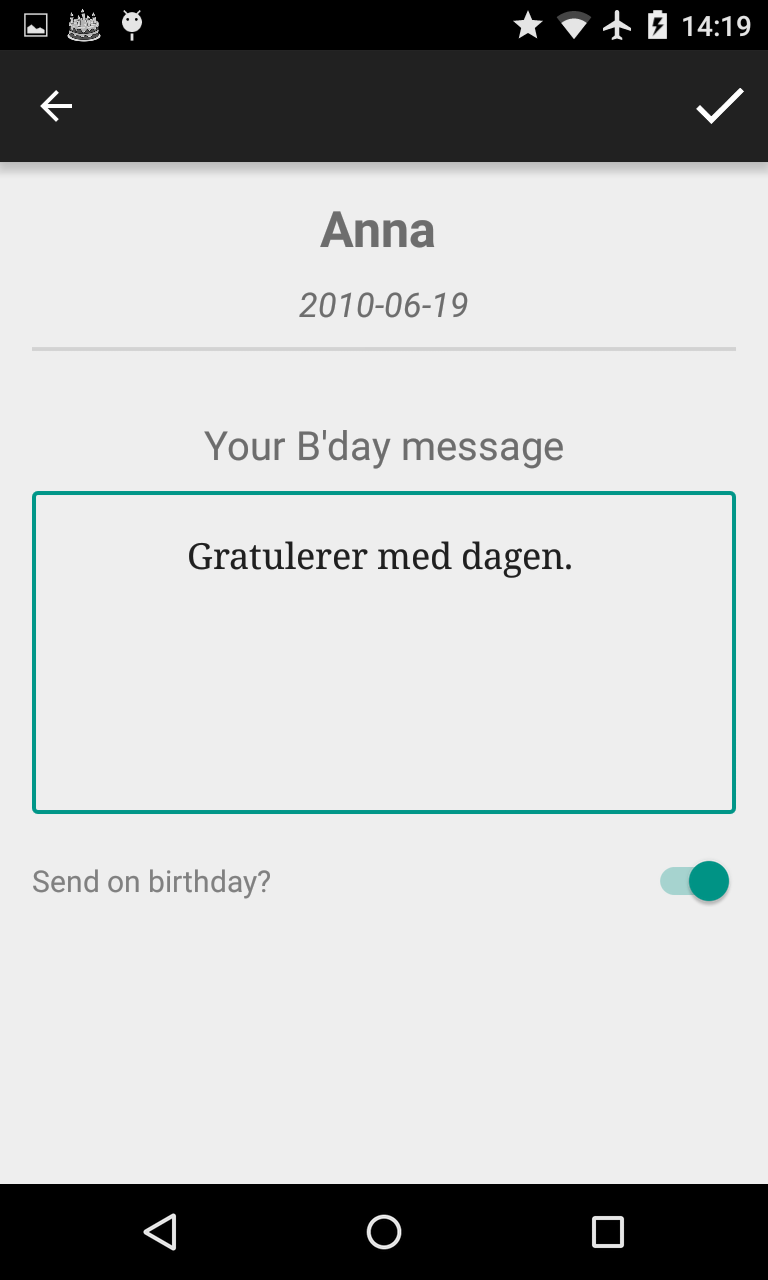
\includegraphics[width=\textwidth]{./img/nexus4/3.png}
        %\caption{Service notification}
        \label{fig:res_meld}
    \end{subfigure}
    \caption[Responsiv design]{\textbf{Responsiv design.} Følgende eksempler viser når applikasjonen kjører på en Nexus 4 med oppløsning på 768 x 1280 piksler. Øvrige bilder i rapporten er fra Nexus S med 480 x 800 piksler. Alle skjermbilder tilpasser seg dynamisk til skjermstørrelsen.}
    \label{fig:responsiv_design}
\end{figure}


\chapter{Hvorfor er dette en god design?}
\begin{description}
\item[Grafisk tema]
Det er enkel å oversiktlig grafisk tema i applikasjonen. Det er ingen skarpe eller påtrengende farver i komponenter elle fonter. Applikasjonen er tilnærmet stylet som en standard applikasjon som er tilgjengelig i API 19.

\item[Responsiv design]
Alle grafisk komponenter er satt opp med en rekke av regler som gjør det mulig å bruke applikasjonen på alle typer av skjermstørrelser. Det er uavhengig for dersom applikasjonen blir brukt på en enhet med liten eller stor skjerm. Hvert element består av statiske komponenter som har sin faste posisjon og dynamiske komponenter som skaleres etter tilgjengelighet for plass. Et godt eksempel på dette er hver rad i listefragment som ekspanderer etter oppløsning på enheten. Dette sikrer tilnærmet samme brukeropplevelse på enheter som benytter seg av større oppløsning på skjermene, se figure \ref{fig:responsiv_design}.

\item[Navigasjon]
Det er enkelt å navigere gjennom aktivitetene gjennom å kun forholde seg til action bar. Alle komponenter er alltid på samme plass og brukeren trenger ikke å lete etter knapper eller andre interaksjons komponenter i det kjørende aktiviteten.

\item[Tilbakemelding]
Brukeren får tilbakemelding om at tjenesten kjører gjennom at det vises en ikon i form av en bursdagskake i activity bar. Ikonen er tilnærmet grå farve for at den skal passe godt inn med andre system ikoner som vises der.

\item[Lagdeling]
Det er klar lagdeling i form av pakker mellom klassene. Det benyttes en repository pattern for klassedelingen som består av blant annet følgende:
\begin{itemize}
\item BLL - business logic layer. Her samles alle klasser som brukes til å på noen måte behandle data som kommer fra og til brukeren eller som benyttes av tjenester. 
\item BOL - business object layer. En pakke for \textit{POJO\footnote{POJO - plain old java object}} klasser som i dette eksempel er klassen Person.

\item DAL - data access layer. En pakke for alle klasse som har med lesing og skriving til og fra databasen å gjøre. Klassene her består av en rekke metoder som returnerer etterspurt data fra lagring.

\item LIB - biblioteks klasse. En pakke for alle klasser med static objekter som konstanter som brukes på tvers over hele applikasjoner eller interfaces. I dette eksempelet er det interfaces som brukes som \textit{callbacks} mellom klasser.

\item briadcasts - samlepakke for Android broadcast objekter.

\item fragments - samlepakke for alle fragmenter som benyttes i aktiviteter aller dialoger i applikasjonen. 

\item services - samlepakke for alle tjeneste objekter som brukes av applikasjonen. 
\end{itemize}

Følgende lagdeling mellom klasser gjør det veldig enkelt å vedlikeholde kodebasen. Det blir ganske så enkelt å for eksempel bytte ut flere av objektene. Et eksempel på dette kan være dersom man ønsker å erstatte SQL tilnærming i DAL pakken med en ORM løsning. 

\item[Fragmenter]
Det benyttes flere fragmenter i applikasjonen hvilket gjør det enkelt å variere innhold i de grafiske delene uten å forholde seg til alt det som medfører bruk av aktiviteter i applikasjonen. 

\item[Validering]
Validering av brukerdata gjør det umulig for brukere å legge i feil data i applikasjonen og med dette blir alt kvalitetssikret slik at for eksempel riktig telefonnummer lagres i databasen.

\item[Stabilitet]
Applikasjonen er godt testet. Under testing har det ikke forekommet noen kræsj. Applikasjonen er testet både på emulator med API 19 samt fysiske enheter med API 19 og API 20. 


\end{description}





\chapter{Veien videre}
\textbf{Følgende avsnitt beskriver noen funksjonalitet og forbedringer som jeg ønsker at skal implementeres under videre utvikling av applikasjonen. }

\begin{description}
\item[Varsler]
I informasjons feltet for telefonen bør det bli vist en melding etter at man har sendt ut meldinger til en person. Dette kan være greit for brukeren som en enkel påminnelse om at hilsen er blitt sendt.

\item[Tidssoner]
Det hadde vært fint å ha mulighet til å spesifisere andre tidssoner for kontaktene slik at man ikke sender melding til noen minst på natten.

\item[Valideringslytter]
Nå blir inputvalidering kjørt samtidig som brukeren klikker på videre knappen. En eventuell forbedring kan være at man validerer så snart et felt har mistet fokus. Slik funksjonalitet vil gi brukeren hyppigere respons på feil input. 

\item[Melding kontroll]
En overordnet struktur som kvalitetssikrer at servicen ikke sender melding til en person to ganger samme dag dersom servicen blir startet om. Dersom man starter om hovedservice f.eks. ved om start av telefonen kommer hovedservice å kjøre dersom tiden for utsendelse er satt tilbake i tid. Dette gjøres ettersom systemet forsøker kjøre servicen dersom systemet tror at servicen ikke har kjørt. Slik funksjonalitet er helt riktig slik at man ikke misser å sende melding en dag også når telefonen blir skrudd av under den planlagdte tiden for sending av meldinger. Det som mangler er at man setter en enkel flagg feks i databasen eller delte innstillinger den første gangen meldingen blir sendt sammen dag.


\item[Custom \texttt{DatePicker}]
Datovelger som brukes nå er begrenset slik at man ikke kan sette dato i fremtiden. Det som kanskje hadde vært med funksjonelt er en data picker som tilbyr kun dag å måned ettersom egentlig er det ikke egentlig nødvendig å registrer fødselsdag for kontaktene uten det eneste som vi trenger er dag og måned.

\item[Historikk]
En enkel form av historikk for hvilke personer som man har sendt meldinger til. 

\item[Import]
Det er flere applikasjoner på telefonen som har en egen \texttt{ContentProvider} og kan f.eks. brukes til å velge kontakter som man ønsker å importere fra telefonens kontaktliste eller apper for sosiale medier.

\end{description}


